\documentclass[final,times]{elsarticle}
\usepackage{framed}
\usepackage{hyperref}
\usepackage{tikz}
\usetikzlibrary{arrows, decorations.markings}
\usepackage[utf8]{inputenc}
\usepackage{graphicx}
\usepackage{subfigure }
\usepackage{verbatim}
\usepackage{amssymb}
\newcommand{\done}{\item[\checkmark]}
\newcommand{\crossed}{\item[$\times$]}

    


\setcounter{secnumdepth}{4}
\setcounter{tocdepth}{3}
\hbadness=99999
 
\graphicspath{ {images/} }

\journal{Intelligent Environmental Data Analysis and Pollution Management}

\begin{document}

\begin{frontmatter}

\title{Aire Guru: Making Pollution Data Accessible, Relevant, and Compelling.}

\author{Luz Morales}
\address{International University of La Rioja}
\ead{luzmoralesjimenez@hotmail.com}

\begin{keyword}
 Air Quality Index \sep Pollution \sep Monitoring \sep Visualization \sep Analysis \sep BigData
\end{keyword}

 \begin{abstract}
Government open data portals make a huge effort to collect data and make it available to their citizens.
However, this data is often wasted, since it is not always in effectively accessible, relevant and compelling
for the average citizen. Air quality data is one such example.

Urban residents are surrounded by many sources of air pollution, and it is the direct cause of many different symptoms, ranging from simple eye irritation 
to, in extreme cases, death. Particularly for high-risk groups like children and the elderly.
The WHO (World Health Organization) estimates 4.2 million deaths
\footnote{\url{https://www.who.int/airpollution/ambient/en/}} per year due to air pollution.
Air pollution has a significant affect on people with asthma, cardiopathies, allergies, and neurological pathologies.

Air pollution not only aggravates existing diseases, but can also be an initial cause of them, such as in the case of foetal brain
damage\footnote{\url{https://tinyurl.com/y2fzk8uk}} 
caused by the mother's exposure to air pollution.

To be able to control the level of exposure we need to know the levels
in the specific locations that we frequent, and the variation during specific times.
To make this information as accessible as possible, it should be freely and publicly available, and the presentation
must be simple enough to be understandable by the average citizen.

We have created a tool - Aire Guru - which collects air pollution data periodically, stores it for historical use, 
processes it to extract relevant information, personalizes it to engage the user with regard to their individual
circumstance, visualizes it in an easy to understand format, and provides it online to facilitate its accessibility. Furthermore,
descriptions of all the data and how it has been processed are also provided to raise public awareness of the value
of this data. Aire Guru has been successfully tested, using the Air Quality data provided
by the Málaga open data portal\footnote{\url{https://datosabiertos.malaga.eu/}} in the Spanish city of Málaga.

There are already many tools available, however they have various failings.

The most common problems are:

\begin{itemize}

\item Obsolete measurements. Measurements need to be taken regularly, since there can be huge differences
between pollution levels at different times of the day.

\item Limited geographic coverage. The data must cover a reasonable proportion of areas that people spend significant time in.

\item Insufficiently granular measurements. Measurements must be at a reasonably fine level of granularity. One single measurement for an entire city is not useful.

\item Poor presentation. Often the information is presented in an uninterpreted form, making it difficult for users to visualize, especially in a geographic sense.

\item Poor discrimination and interpretation. Many tools show individual values as a number or a colour. This information is not
enough for the user to take control of their exposure. Such visualizations are not really compelling. 

\end{itemize}

Our webtool \footnote{\url{https://airquality.guru/}}, solves the deficiencies described above.

Measurements are published hourly and come from measurement stations placed throughout the 
city of Málaga, covering entire urban region at a granularity of $100m^2$

The information is presented in a clear and simple manner, making it possible to see the most polluted regions,
and allowing the user to make comparisons both geographically and historically. It provides personalised information, such as the most relevant pollutants for a user's particular medical conditions, and can track
the pollution they are exposed to both in real time and over a historical period, by linking with location data from their mobile device. 

The system has been successfully tested with 14 subject in the Spanish city of Málaga. The survey showed a high degree of satisfaction, particularly regarding the clarity and completeness of the the information and analysis.
More than the half of the subjects were not aware of how air quality is measured and how it 
can affect their health. Four of the subjects discovered that they have a medical 
condition which can be affected by air pollution.
    
Aire Guru is available online, free of charge. 
\end{abstract}   


\end{frontmatter}

\begin{comment}
\newpage
\tableofcontents
\listoffigures
\end{comment}
\newpage

\section*{Introduction}
\subsection*{}
--Info out the abstract
\subsection*{Motivation}
Con el paso de los annos hemos visto en el procesado de los datos una oportunidad de oro, 
tanto para mejora nuestra vida diaria como para intentar predecir
eventos futuros. Por esta razon, surge la tendecia de almacenar todos los datos que tenemos 
a nuestro alrededor con la esperanza de que algun dia sean tratados.
Como por el momento no tienen ningun fin en concreto, se almacena competamente todo, sin discriminacion.
Sin saber si en algun momento seran utiles o no.\\

Por otra parte, multiples empresas tanto publicas como privadas, incluidas nuestros gobiernos, 
en su compromiso por la transparecia y/o esperanza de sacarle provecho, publican estos datos 
periodicamente.\\

Aunque estos datos esten disponibles para todos los usuarios, no significa que sean provechosos para el 
usuario medio, ya que se enfrenta a multiples retos.\\

En los siguientes apartados se realizar un recorrido por las etapas necesarias para hacer estos datos
accesibles, relevantes y atractivos para el usuario medio.
El objetivo de este capitulo es estipular los puntos necesarios para usar los datos de una manera provechosa y
que nos ayude en nuestro dia a dia de una forma util. Estos conceptos se han aplicado en el proyecto Aire Guru, 
que acerca los datos a los usuarios de una manera facil, amigable, compresible y adaptados a sus necesidades.\\

Aire Guru es una herramienta web para la monitorizacion personalizada de la calidad del aire en Malaga.



\subsection*{Structure}

In this chapter we will see how to make the data accessible, relevant and compelling for 
the average user. For each one of the secluded ones, we will see the theory, as it has been applied
in the Air Guru project and its evaluation.
Next, we will see a general evaluation of these three concepts and to finish the 
obtained conclusions.
This chapter is written with the objectives we want to achieve in mind for the reusing of bigData. It means, make the 
concepts accessible, relevant and compelling. It intents to be a guide which show these principles
in its structure.




 
\newpage
\section{Accessible}

Los datos se consideran accesibles por el usuario cuando este no necesita realizar un esfuerzo desmesurado para
poder obtenerlos, entenderlos y usarlos, es decir, aplicarlos a su situacion particular. Para lograr estos objetivos,
es necesario que el usuario pueda acceder a ellos de una manera que le resulte familiar y en un lenguage y nomenclatura
que pueda entender.\\ 

En este apartado veremos si es posible el acceso a los datos por un usuario medio y como optimizar la accesibilidad.

\subsection{Availability}
    
As we mentioned in the introduction to this chapter, the dataSets may be available in the original source. However, this doesn't necessarily
mean that they are readily accessible.
The challenges we encounter with the raw data direct from the source of origin, are the following: \\   
 
\textbf{Location}. DataSets are usually available in open data portals that have been organized and structured in particular ways.
Despite more companies attempting to offer functional and efficient user interfaces, often a complicated search and selection process is necessary for a user to find what they need. Sometimes the data may not all be available in the one location, but may require searching through multible portals.
\textbf{Extraction}. DataSets are usually available through an API (Application Programming Interface). APIs are not easily interpretable by the average user. Normally there will be a document describing the fields and values presented, and indicating how to actually use the API. \\

\textbf{Readability}. DataSets are usually represented in a format designed to be processed by software. This is fairly unintelligible to a human user. At best,
the data will be represented in a table and even then, it will often be quite difficult to extract the required information.

Therefore, we can not say that data interfaces are commonly accessible in a useful way for the average user. \\

\subsubsection{How can we solve the problem?} 

We must provide the information required by the user in an uncomplicated manner, in a format that is easy to read and interpret, and we must describe it in a way that is easy to understand and quick to digest..

In order to collect the information which is relevant to the user, we will need to carry out processes such as extraction, transformation and
data cleaning.
 
\subsubsection{How we solve it using Aire Guru.} 

Our tool uses the air quality data provided by the city of Malaga in its open data portal.\footnote{\url{https://datosabiertos.malaga.eu/}}\\
\begin{figure}[ht]
    \centering
   \subfigure[Main page]
    {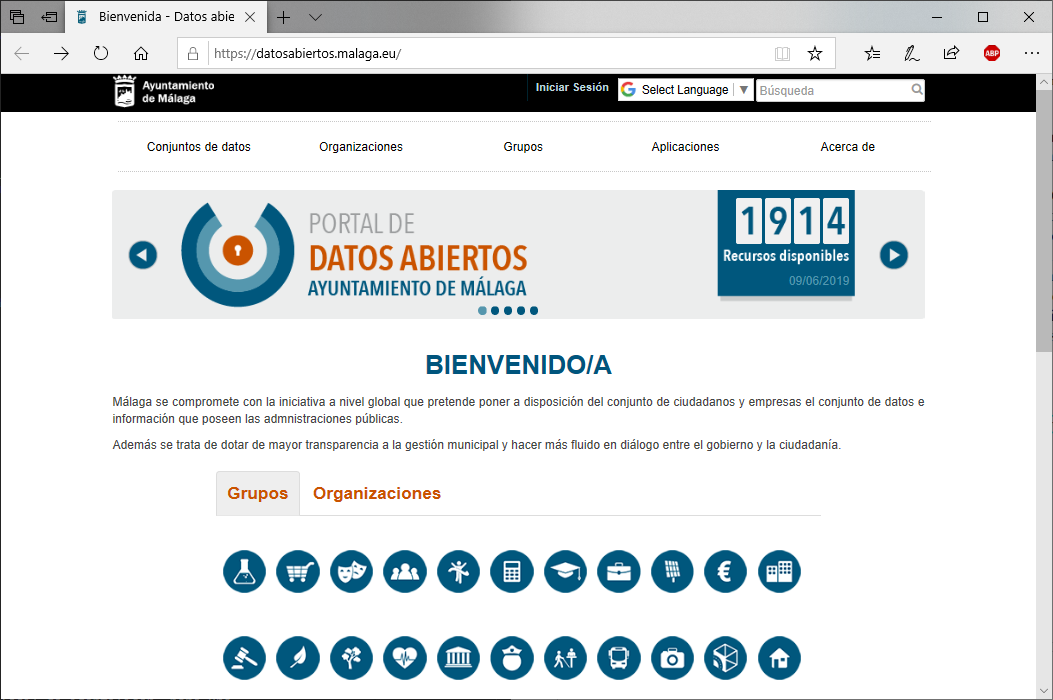
\includegraphics[width=5.5cm]{openDataPortal}}
    \hfill
    \subfigure [Category environment]
       { 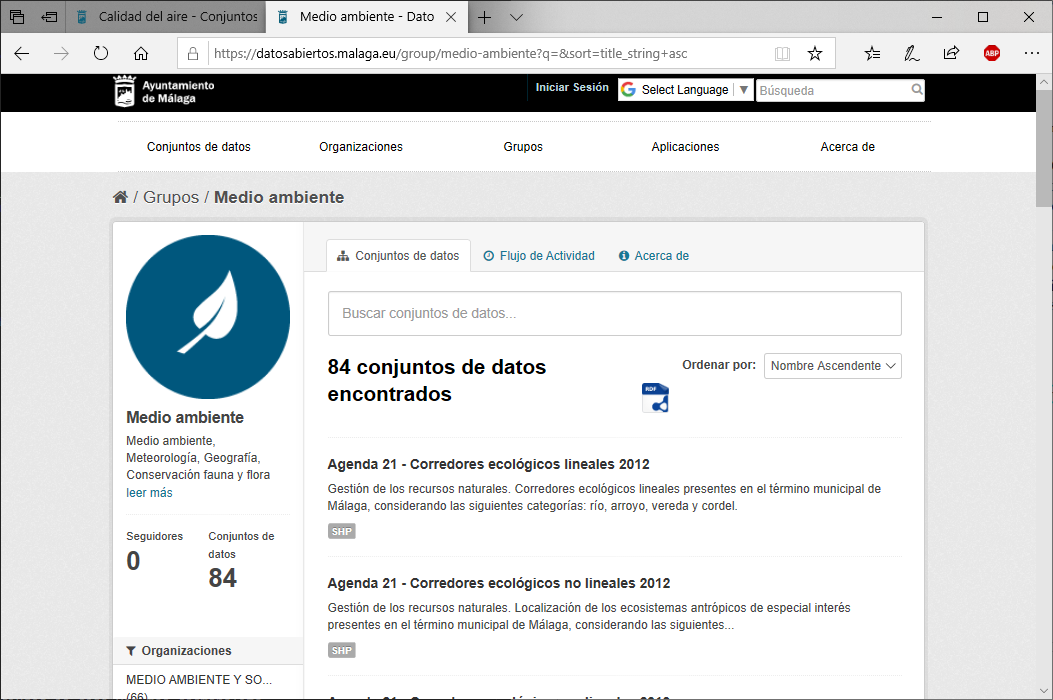
\includegraphics[width=5.5cm]{openDataPortalEnviromentCategory}}




    \vfill
     \subfigure[GeoJson Document]
     { \centering 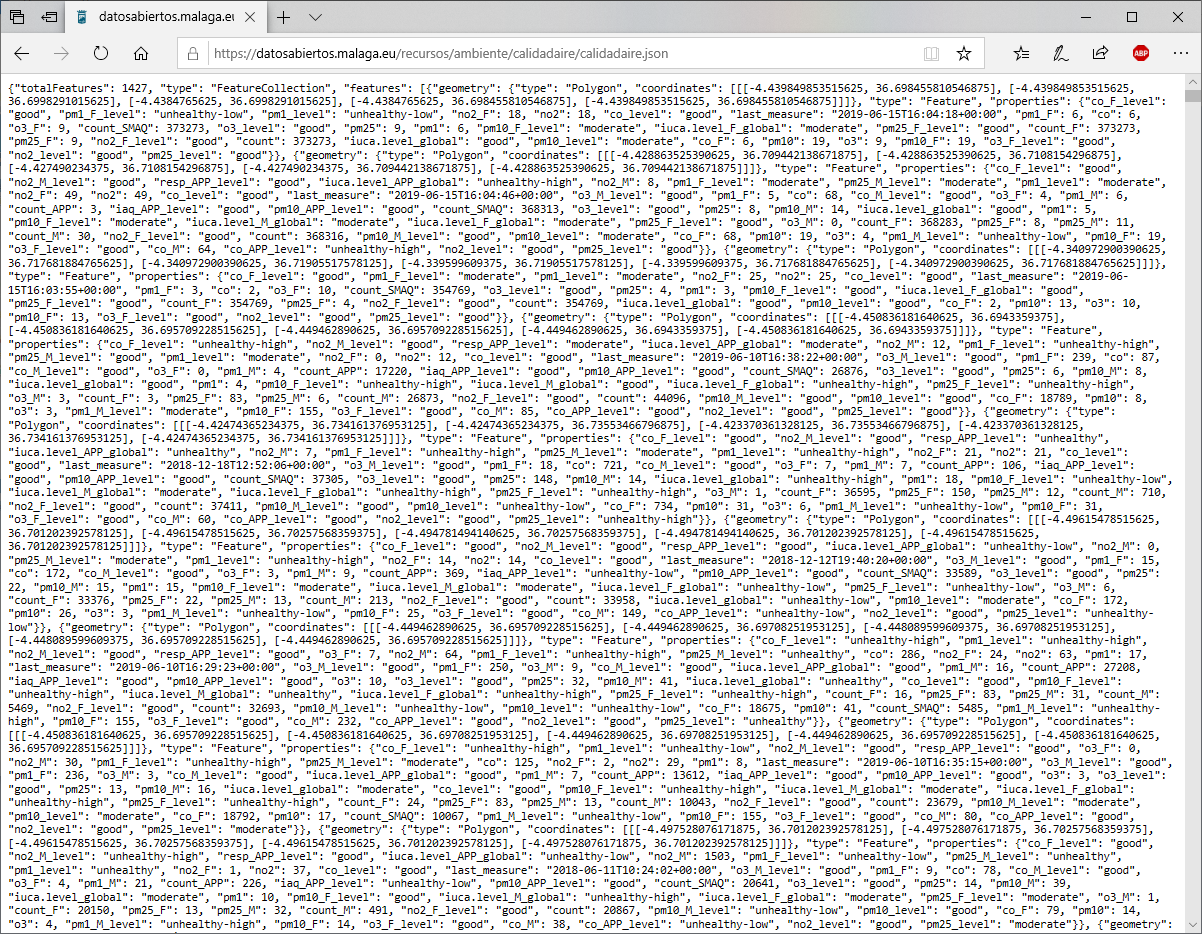
\includegraphics[width=4.75cm]{geoJsonAirQualityDataRaw}}
  
  \caption{Open Data Portal Malaga}
    \end{figure}

    This data portal offers a variety of categories (represented by different icons) indicating classifications of the dataset.
    Once a category is selected, the user is presented with a search bar that allows them to search for specific data using keywords.\\
    
    In this case, if we click on the link, data is displayed in a new tab. The use of software
    for translating the data is not strictly necessary, but we can see that the format (JSON) is not easily readable in human terms.

Aire Guru \footnote{\url{https:\\aire.guru}} offers all the necessary information on a web platform which has been designed to facilitate human understanding.

\elsparagraph{Evaluation}  

\begin{itemize}
    \done Location. Finding data is made simple, since information is displayed immediately on accessing the website. The main page
         presents the levels of pollution in all areas without the need to make any selection.
    \done Extraction. No specialist software or computer knowledge is necessary to access the information.
    \done Readability. Aire Guru includes a map which shows pollution levels, represented by different colors. These colors are defined by a legend
         below the map. It also includes a glossary explains the concepts presented on the website, the meaning of each section and includes clear instructions on how to
         use and navigate through the web page.
 

\end{itemize}
\newpage

 



\subsection{Know about}

No matter how optimized the representation of the data is and how available we make it, if users are not aware
 of the existence of the resource, they can not use it.

\subsubsection{How to solve it} 
The best way is to advertise the product in the right media with right format.
\subsubsection{How we solve it. Aire Guru} 
Our tool is implemented for the city of Malaga, so we are currently working to publicize it in this city.
It is currently available in the open data portal in the web site tab \footnote {\url {https://datosabiertos.malaga.eu/aplicaciones}} \\
Aire Guru participated in the first open data reuse contest organized by the Malaga City Council \footnote {\url {https://tinyurl.com/yx9wzutj}}
and was a finalist in the web page category.


\begin{figure}[ht]
    \centering
   \subfigure[Advertising in the open data portal of Málaga]{ \centering 
\includegraphics[width=6cm]{aireGuruFinalist}}
   \hfill
   \subfigure[Finalist]{ \centering 
\includegraphics[width=5cm]{aireGuruFinalistCertificate}}
 
    \caption{I Contest of reuse of open data. Malaga's town hall}
    \end{figure}

\elsparagraph{Evaluation}  
\begin{itemize}
    \done It is currently published in the open data portal of the City of Malaga.
\crossed More work should be done on advertising the platform and making it known.
\end{itemize}
\newpage
\subsection{Interpretabilidad}
The platforms provide a huge volume of data, since, as mentioned earlier, they collect as much data as possible.
There will be multiple samples containing the specified set of fields. These field sets may be similar to each other but don't need to be identical.
From this data, we need to select the relevant samples, and from these, the fields necessary to represent specific information.


Below we can see examples. The first one is taken from the European open data portal
\footnote{\url{https://tinyurl.com/y3d76525}} and the second from the North American open data portal
\footnote{\url{https://data.cityofnewyork.us/api/views/kku6-nxdu/rows.json?accessType=DOWNLOAD}}.

\begin{figure}[h]
    \centering
    \subfigure[EEUU Open Portal.Demographic Statistics By Zip Code]
     {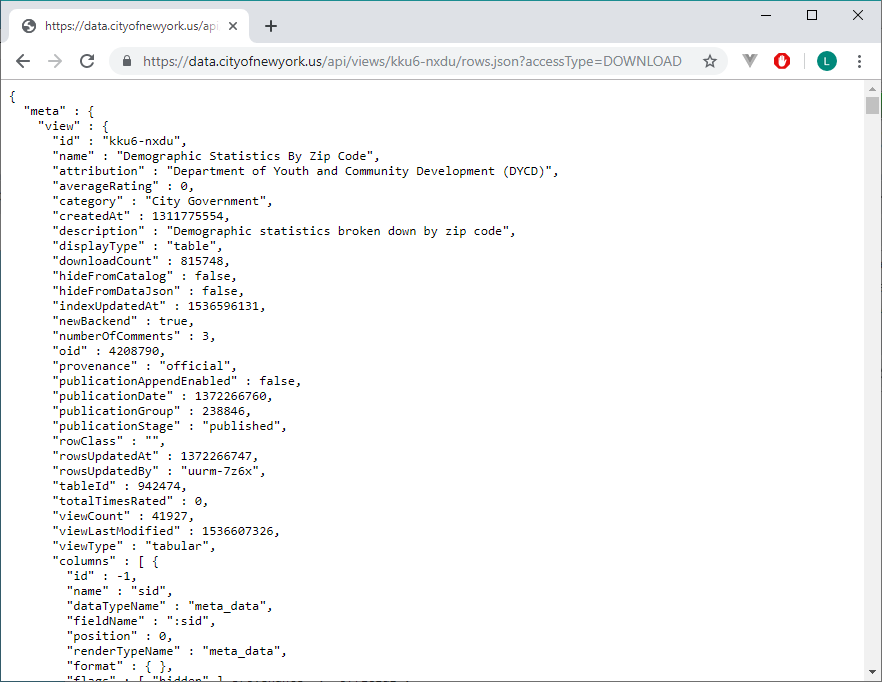
\includegraphics[width=5cm]{ExampleOpenDataEEUU}}
    \hfill
     \subfigure[European Open Data Portal. Air pollutant concentrations 2015]
    {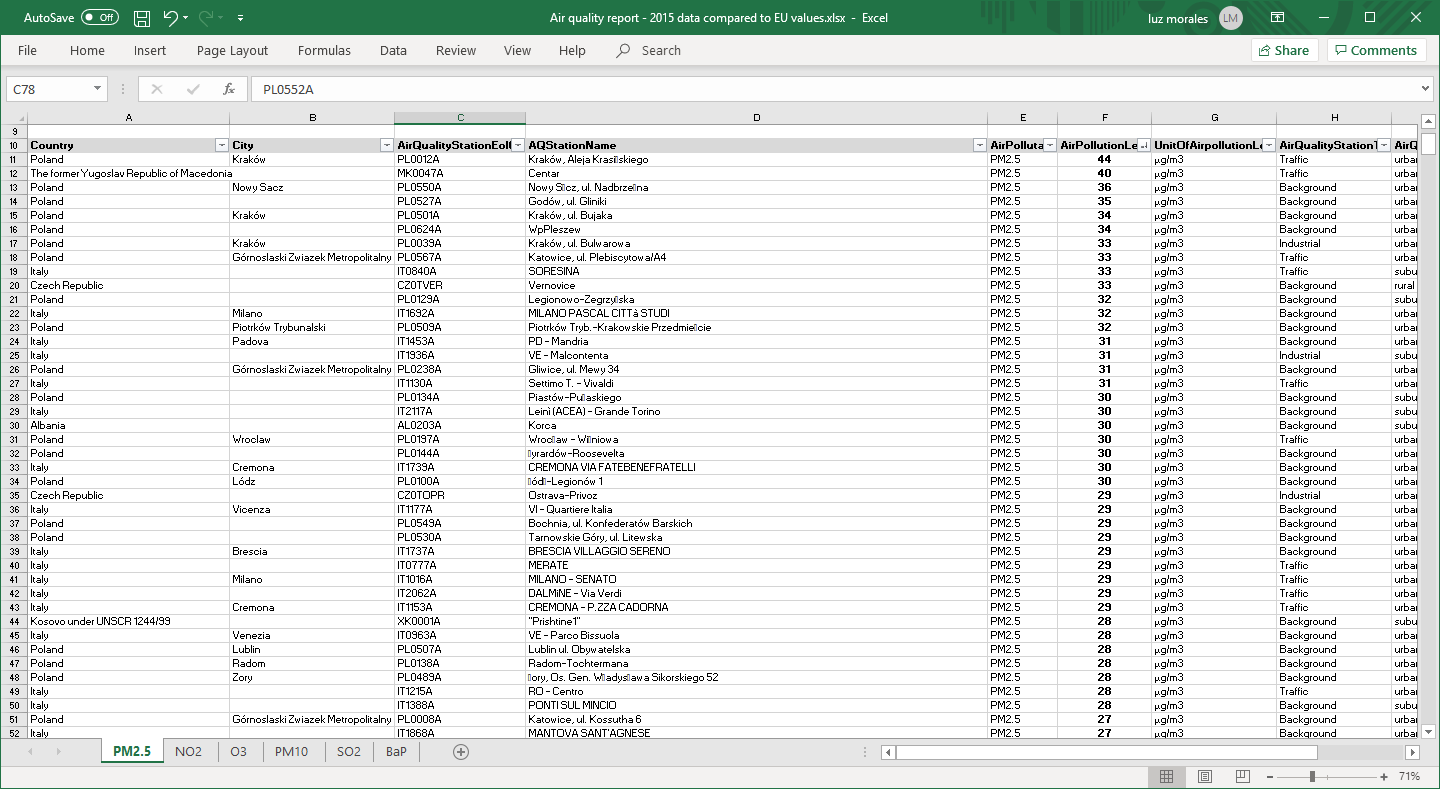
\includegraphics[width=7cm]{ExampleOpenDataEuropean}}
    \caption{Open Data Examples}
\end{figure}

    

    
\subsubsection{How to solve it} 
We obtain our required data through a series of processes such as extraction, transformation and
cleaning of the data. Without automation, theses processes are tedious and time consuming. 

\subsubsection{How we solve it. Aire Guru} 

The extracted data is in GeoJSON format, a format which provides a JSON object with nested subdocuments. Each of these
subdocuments contains a set of data in key-value form.
In the following figure we can see the beginning of the document downloaded on June 9, 2019
\footnote{\url{https://datosabiertos.malaga.eu/recursos/ambiente/calidadaire/calidadaire.json}}\\
\newpage
\begin{figure}[h]
    \centering
   \subfigure[First subdocument]{ \centering 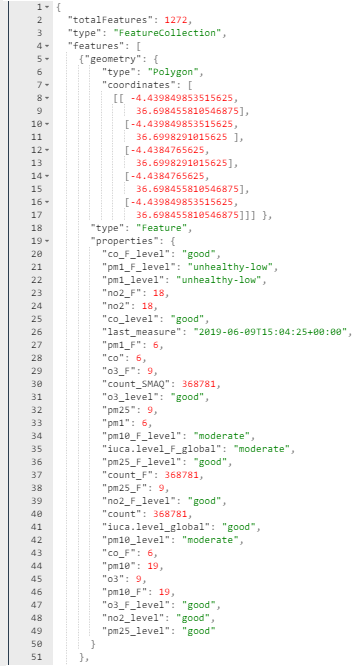
\includegraphics[width=4.75cm]{geoJsonAirQualityData1}}
   \hfill
   \subfigure[Second subdocument]{ \centering 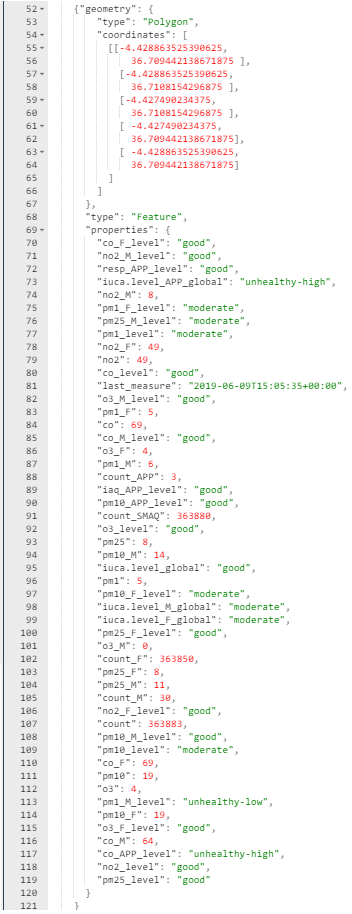
\includegraphics[width=4.75cm]{geoJsonAirQualityData2}}
 
    \caption{Air quality Document [09/06/2019].Open Data Portal Malaga}
    \end{figure}
    
    In this excerpt we can see the first two subdocuments. Each subdocument contains the coordinates of the air quality 
    measuring station, the date and time when the measurement was recorded, and the values of the measurements.
    In the following figure we can find the description provided by the open data portal.
\begin{figure}[ht]
    \centering
    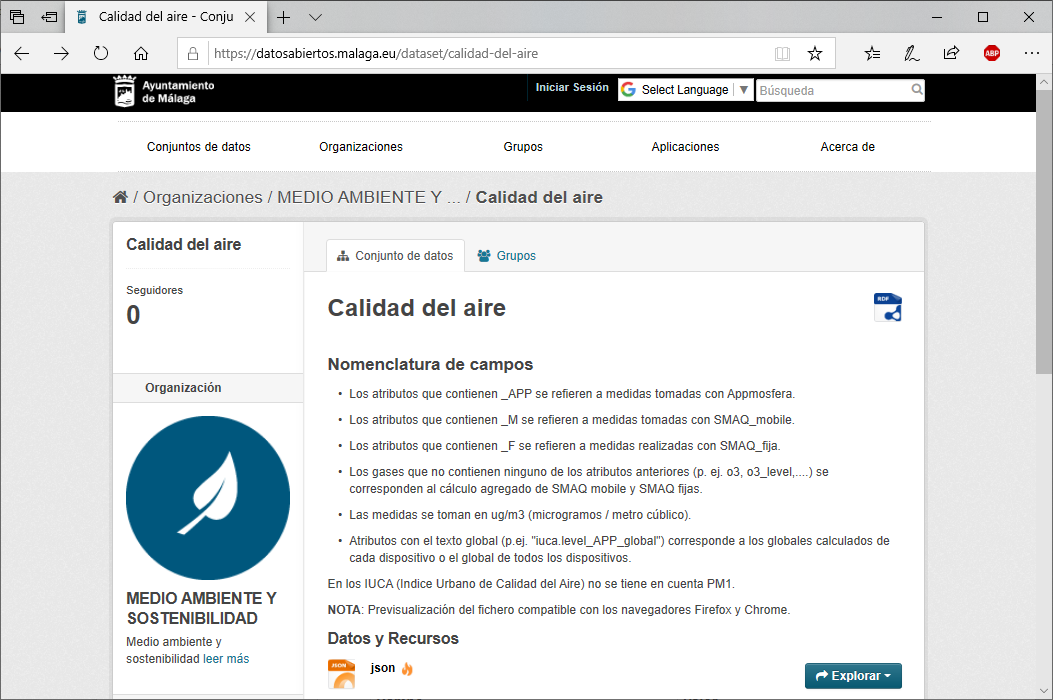
\includegraphics[width=8cm]{geoJsonAirQualityDataDescription}
    \caption{Air quality data description [09/06/2019].Open Data Portal Malaga}
\end{figure}


For a more detailed description of the measures, we have to resort to an external resource. In this case we directly contacted 
the company that installs the UrbanClouds\footnote{\url{https://urbanclouds.city/es/}} measuring stations and provides the data 
to the Malaga city council.

After selecting the necessary fields according to our design plan, we carried out different cleaning, transformation and extraction tasks. \\


\textbf{Cleaning}. We need to eliminate the repeated or non-relevant fields. For example, the identifier of the measuring station is 
unneccessary as the  already contains the coordinates of the station, and coordinate representation is more interesting for our purposes. \\

\textbf{Transformation}. We need the values to have a format appropriate to the fields that they represent. For example, the date and time 
of the measurement is stored in date format
instead of the string provided in the raw dataSet. \\

\textbf{Extraction}. We need to select the relevant fields. This dataSet offers one or more measurements for each pollutant, which can be 
represented by three different fields, a
quantitative measurement, a qualitative of the fixed station of measurement and a qualitative station of a mobile station. We will add a 
field containing the measurement which is most relevant for our purposes, and eliminate the non-relevant measurerments to minimize processing time. \\

For security, a second totally independent architecture has been implemented that collects and stores the raw data.

\paragraph{Evaluation} \mbox{} 
\begin{itemize}
    \done We can understand exactly what each one of the fields represented in the dataSet means thanks to the 
         complementary information presented in the open data portal and by the complementary information provided by the company in charge of
         collect the data.
    \done The data needed for our model has been extracted from the raw data.
    
\end{itemize}
\newpage

\subsection{Modelo}

Recall that the main objective of accessing the data is to obtain knowledge, to understand and make sense of it. Of course, 
pure data by itself has no value until we can understand it and apply it. We must contextualize, process, and analyze the 
information to gain useful knowledge. \\
    
\begin{figure}[ht]
    \centering 
    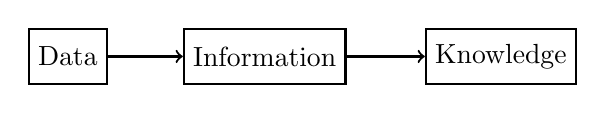
\begin{tikzpicture}[thick]
        \node[draw,rectangle,minimum size=20] (a) {Data};
         \node[draw,rectangle,minimum size=20,right of= a, node distance=2.5cm] (b) {Information};
         \node[draw,rectangle,minimum size=20,right of=b, node distance=3cm] (c) {Knowledge};
         \draw[->] (a) to (b);
        \draw[->] (b) to (c);
     
      \end{tikzpicture}
      \caption{Diagrama. De datos a conocimiento}
    \end{figure}
 
    In order to obtain this knowledge, the user must correctly interpret the data. It's not enough to know what the values and 
    units individually represent, but what they mean in the big picture. For that the user must already have expertise in the 
    area, or must engage in further research allowing them to understand the data that has been extracted.
     
    In order to build a system that makes data accessible, it is essential to design a model to specify the
    information that we want to obtain. The design of a system will allow that, based on given values, provide some results.
    For this it will be necessary to have a solid knowledge of the dataSet that is needed, the values,
    their units and how they relate to each other.


\subsubsection{How to solve it} 
Study the objective sought and resort to the help of experts if necessary to acquire the necessary knowledge
on the subject. Design a model that provides the information we are looking for.

\subsubsection{How we solve it. Aire Guru} 
Aire Guru aims to increase the awareness of the level of pollution that surrounds us. To do this, it uses a measure called
the air quality index (AQI), specifically the European air quality index (EAQI).


\newpage
\begin{figure}[ht]
    \centering
    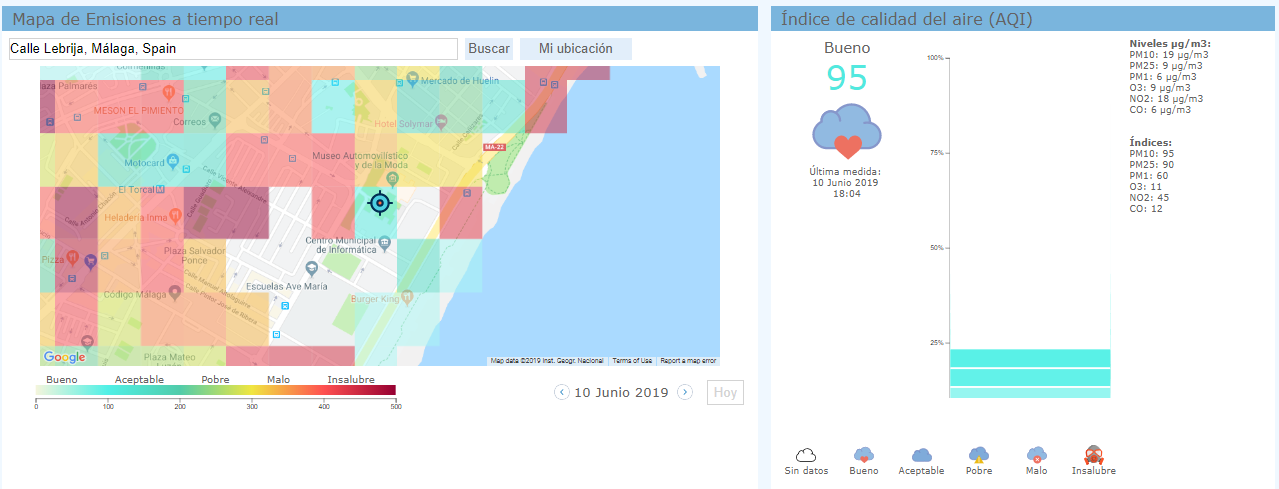
\includegraphics[width=10cm]{mapAireGuru}
    \caption{Aire Guru. Landing page. Top section}
\end{figure}

It shows the AQI in the whole city of Malaga by zones, both the general and the AQI of each of the 
pollutans in a more disaggregated form from September 2018 to the present. It also shows the evolution
of these for days, months and years.
It is capable of creating a set of the most relevant pollutans by medical condition. An innovative feature is the capacity to display levels of any particular pollutant by hour, day, month, or year. 

\elsparagraph{Evaluation}  

\begin{itemize}
\done The information is focused on an objective, informing the user of the level of pollution that surrounds them, both  in real time
and in the past.
\done The information follows a logical thread; it tells a story.
\done The web offers understandabl, useable information, not just raw data.
\end{itemize}

\newpage
\subsection{Formato}
El punto clave para que el usuario entienda lo que queremos transmitirle es crear una comunicacion fluida entre la representacion
de los datos el usuario. Para ello  deberemos asegurarnos que hablamos el mismo idioma, con un vocabulario facil de entender y
con proximidad, es decir,dejar la terminologia a un lado y comunicar el objetivo de la manera mas simple posible.
Por ello la representacion de la informacion jugaran un papel fundamental para que la 
informacion sea absorbida por el usuario de una manera natural.


\subsubsection{How to solve it} 
Este modelo debera proporcionar la informacion al usario en un lenguaje o formato compresible. Si no es posible proporcionaremos las 
herramientas necesarias para que este pueda comprender el contexto de la informacion.
Deberemos estudiar que tipo de representacion es mas adecuada, no siempre una grafica es la representacion mas adecuada, deberemos hacer un 
estudio de tanto al publico al que va dirigido como como podemos acentuar la informacion que sea mas relevante en la manera 
correcta.
Si nos declinamos por realizar una representacion con graficas, deberemos estudiar los datos para saber que tipo de grafica. Por ejemplo, 
si hablamos de muestras y queremos saber la densidad, nos inclinaremos por un grafico de densidad y si por ejemplo buscamos la diferencia 
entre sexos, utilizaremos un grafico de tartas.

\subsubsection{How we solve it. Aire Guru} 
La herramienta Aire guru presenta la informacion en el idioma nativo de la ciudad y se utiliza un lenguaje sencillo y directo.
See utiliza el mismo estilo, colores e iconografia en todo el diseno para que el usuario se familierize rapidamente y pueda
prestar atencion al significado de los datos en vez de perderse en el diseno e intentar encontrar su significado.//

Unos de los objetivos es representa la contaminacion por zonas de la ciudad, por lo que se ha utilizado un mapa sobre el que se representa
 el AQI general calculado. Este es un formato mas legible para los usuarios ya que no tiene que trabajar para realizar una imagen visual
 de los distintos lugares de la ciudad. Este indice mustra un indicador con cinco niveles representados por una escala de colores desde el 
 turquesa hasta el rojo ("Bueno" "Aceptable""Pobre" "Malo" e "Insalubre"). La razon de esta eleccion es porqu eson los colores oficiales y 
 asi se evita crear confusion al usuario.
 \newpage
 \begin{figure}[ht]
    \centering
    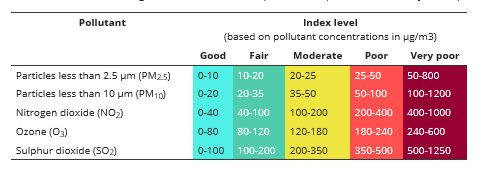
\includegraphics[width=12cm]{EAQI}
    \caption{EAQI Levels}
\end{figure}

Nuestra plataforma introduce ademas una iconografica para ayudar al usuario a tener una idea directa de la situacion, ya que son mas 
explicativos que los colores. En caso de peligro, queda bien representado con el color rojo, pero en el caso del azul o verde, en nuestra cultura, no
tenemos definido un estado para estos colores.\\
\begin{figure}[ht]
    \centering
    
\includegraphics[width=10cm]{EAQI_Icons}
    \caption{Iconografica Aire Guru}
\end{figure}

Para las graficas que muestran variaciones en el tiempo, se han utilizado graficos de lineas, que son las mas apropiadas para este tipo de datos,
ya que muestran la continua evolucion durante un periodo de tiempo. Para representar los distintos componentes del AQI se ha utilizado un
grafico de barras apiladas, ya que se ve que proporcion del AQI total esta formada por que contaminante.\\
\begin{figure}[ht]
    \centering
    \subfigure[AQI Evolution]
     {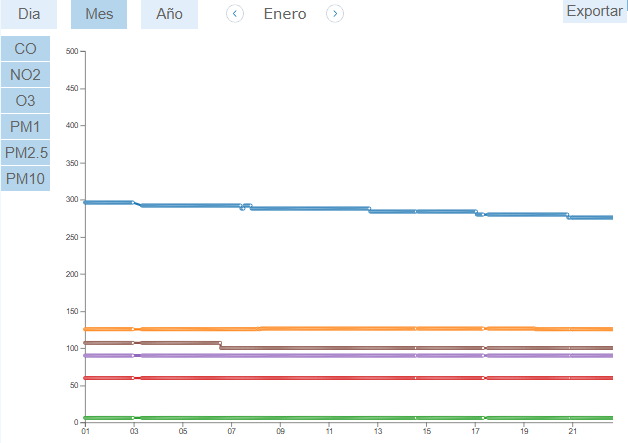
\includegraphics[width=5.75cm]{lineChart}}
     \hfill
     \subfigure [AQI components]
    { 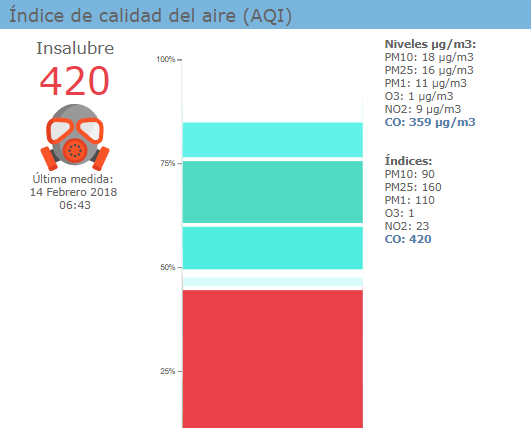
\includegraphics[width=5.25cm]{stakedBarChart}}
 
    \caption{Charts}
\end{figure}

Ademas, para explicar el concepto de AQI y crear un awarnes sobre la influencia que tiene en nosotros la polucion del aire, Aire Guru proporciona un 
glosario y una ayuda con las descripciones de los agentes contaminantes, complicaciones medicas, fuentes de contaminacion, la iconografia utilizada y
una explicacion sobre que es y como se calcula el AQI.\\

 
\elsparagraph{Evaluation}  
\begin{itemize}
    \done El lenguaje utilizado en toda la herramienta es un lenguaje comun, huye de la terminologia cientifica pero proporciona la informacion
    suficiente para enteder la situacion.
    \done Se han estudiado y utilizado las graficas mas apropiadas para cada tipo de datos.
    \crossed Algunos terminos especificos no se han podido sustituir como "Indice de calidad del Aire".
    \done Se han proporcionado la herramientas necesarias para entender el concepto. Se ha utilizado la norma europea de calidad del aire para 
    representar los valores y se ofrece al usuario recursos en la pagina para su comprension ademas de recursos extenos.
    
\end{itemize}
 

\newpage
\subsection{Convenience}
As we mentioned earlier, our goal is for the user to have direct access to the data without having to deal with any
of the technical processes involved in implementing a collection system. The points we must cover to achieve this goal are: \\

\textbf{Infrastructure}. Data collection, processing, storage and visualization. For example, in most cases, the data is
published periodically, but the set of published data only contains the most recent samples. There is no way to obtain
a history of the data if it is not collected, processed and stored periodically. \\

\textbf{Automation}. As we commented in the previous point, these tasks are repetitive and arduous processes, so it will be
necessary to automate, otherwise the effort required by the user to extract the information is not worthwhile. \\

\textbf{Availability} To offer the information to users in a direct way, we should use a platform with which the user is already 
familiar. For example, it is more likely that the user will want to access the data if there are no extra obstacles such as needing 
to install new software on their devices. \\

\subsubsection{How to solve it} 
We will have to provide all the afore-mentioned infrastructure which can collect the data and offer it to the user in an accessible, relevant and compelling way.
We will try to free the user from repetitive actions, we will automate all possible processes, to make the information available immediately.
We must offer the information through a platform with which the user is familiar, nowadays the use of websites or mobile applications is very common.
We must not make the user perform complicated steps, or require them to add extra software or hardware.

\subsubsection{How we solve it. Aire Guru} 
Malaga's air quality dataset is updated every hour, Aire Guru automates the process of collecting the
data through a CRON job that executes a script implemented in JavaScript periodically. This reads the data from the url, processes it,
cleans and stores it in a MongoDB database. That is to say, Aire Guru implements all the necessary collection processes.

Thanks to this infrastructure, the user is able to visualize the evolution of pollutants since 2018. The user can also track their personal exposure
 to these pollutants over the same period of time.

In addition, this automation allows the user to visualize the pollution in the city of Malaga in real time, and see specifically the location where he is 
occurring. \\
\newpage

\begin{figure}[ht]
    \centering
    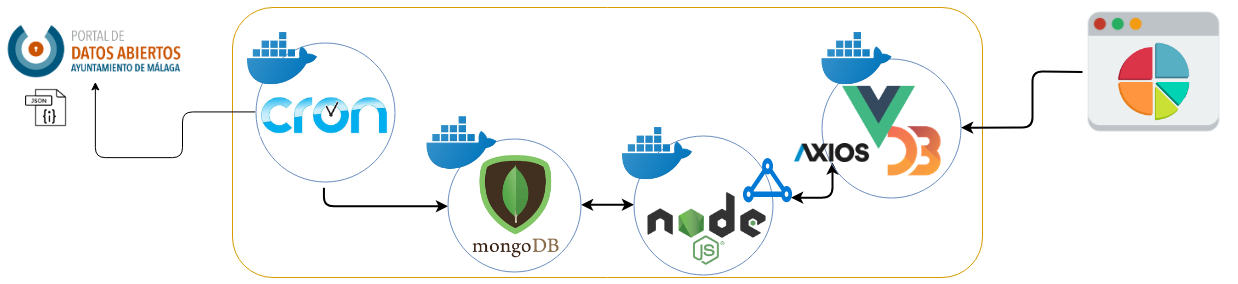
\includegraphics[width=12cm]{aireGuruArquitecture}
    \caption{Arquitecture Aire Guru}
\end{figure}

The data to the users through a web interface. \\

\begin{figure}[ht]
    \centering
    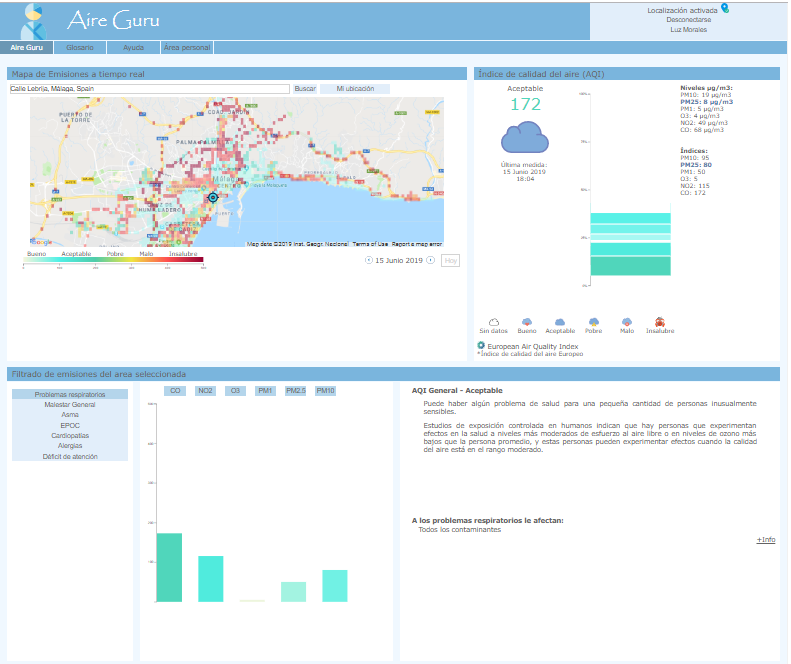
\includegraphics[width=9cm]{aireGuru}
    \caption{Aire Guru. Web Interface}
\end{figure}

To enable access by the majority of the population, Aire Guru is available at the web addresses https://www.aire.guru and https://www.airquality.guru.
We use SSL that guarantees the encryption of data through the network and ensure the user has access to it since, as more and more browsers try to protect 
users by only showing pages that use a secure method.

As we commented previously, all users can see the basic information without having to provide any data or identify themselves, without the need to
perform downloads or installations. Today, almost everyone is familiar with web browsing and if we do not force the user to realize extra taks, as 
requiring them to sign in or install extra software, the probability the user uses our platform will be higher. 

\newpage
\elsparagraph{Evaluation}  
\begin{itemize}
\done The data necessary for our model has been extracted from the raw data.
\done Infrastructure. Aire Guru implements all the necessary architecture of storage, processing and visualization so that the user only has to consult
the data.
\done It automates the processes of data collection and the necessary calculations to show the information to the user.
\done It offers users a free web page, and facilitates the users direct access to information.
\end{itemize}



\begin{figure}[ht]
  \centering
  \framebox{
  \vbox{\begin{tabbing} 
  Check List \\
  \hspace*{10mm} \ding{47} Point 1 \hspace*{25mm} \= \ding{47} Point B \\
   
  \end{tabbing}}%
  
  }
  \end{figure}

    
 
\newpage
\section{Relevant}
 

A good representation of the data does not consist in presenting all of them so that the user has as much information as possible,
It consists in showing you the necessary data so that you can make a direct reading of the situation.\\

In this section we will see the refining of the data to offer the user a relevant and quality information.

\subsection{Design}
To make a good selection in the dataSet of the fields that are relevant or the combination of these, it is essential to
solid knowledge on the subject to be treated. Therefore, it is fundamental to dedicate the necessary time to enter the
importance of the concept, what benefits it can bring or what situations can dameage us.
The points that should be clear in the design phase are: \\

\textbf{Objective}. Conceptually, what problems do we want to solve or clarify. It is very important that we have a clear objective,
     Even if we do not have prior expertise in the subject, having a well-defined objective helps us find the solution, or
     at least enables us to describe it more clearly to the expert who can solve the problem. \\

\textbf{Important points. Notable situations}. As we mentioned earlier, our goal is not to show all the values, but
     which is about providing the user with important information in order to discover the significant situations that influence the
     us, either positive or negative. At a more technical level, it would be the limits or values of what data are those that provide us with information
     of an exceptional situation, or the values that we are trying to identify more easily. \\

\textbf{Data workflow}. When planning the flow of information, it must be clear how to get from one point to another. For example, 
we should start simple and move to more complex representations.

\subsubsection{How to solve it} 
Once a goal has been set, we must stipulate the necessary fields of the dataSet that we need. That is, we select the fields that interest us. 
Following this, we need to analyze the data provided and see if the list of fields that the source offers us is sufficient to rech the chosen objective.
If not directly, we the combination of them. Next, we decide which values are more outstanding and we will provide them to the user.

\subsubsection{How we solve it. Aire Guru} 
Our main objective is to create awareness of the importance of air pollution in our health. For this we investigate different concepts:
\begin{itemize}
    \item What diseases are affected by air pollution
    \item What pollutans are those that create or influence diseases
    \item What are the sources of each pollutant?
    \item What is the representative measure of the level of air pollution.
    \item How it is calculated and what parameters we need for its calculation
    \item What are the harmful levels in general and for each pollutant
\end{itemize}
The measure that best represents the level of air pollution, in this case is the AQI. The city of Malaga is covered by the European legislation, 
so we focus investigations of official sources in this regulation.
We look for the relationships that pollutants have with different diseases, for this we resort to clinical studies. For each of the diseases, we 
research at the symptoms and how they can be aggravated by each pollutant.
For each pollutant, we look for sources of pollution and see if they occur in the city of Malaga and in what concentrations.
With all this information we define that the pollutants that affect air quality are CO, NO2, O3 and PM (Particulated Material). Dfferent levels of particles
affect different diseases in different ways. \\

As the main objective is awareness, we provide all the data in an organized way in the Glossary of Air Guru. \\

Once these pollutans are selected, we verify if we have the particular data in our dataSet. As we mentioned earlier, some samples show measurements 
from fixed and / or mobile stations and these can be quantitative or qualitative and others can be incomplete. We will have to select the
samples to provide us with the most complete information or the most accurate, in this case the quantitative measure will prevail to the qualitative 
one and in the case that there is only qualitative
the following values are decided: Good: 50, Acceptable: 150, Poor: 300, Bad: 400, Unhealthy: 500 and the user will be informed when the value is qualitative. \\


At this point we know how air pollution affects our health, We make very clear which are the undesirable values by using the alert colors, yellow, orange and 
red. These colors are chosen in the palette of the colors provided by the EAQI.
Height is used in graphics, since it is an intuitive representation for humans. In addition, the icon that represents unhealthy levels of pollution, is
totally different, designed to clearly convey danger. \\
\newpage
\begin{figure}[ht]
    \centering
   \subfigure[BarChart Aire Guru]
    {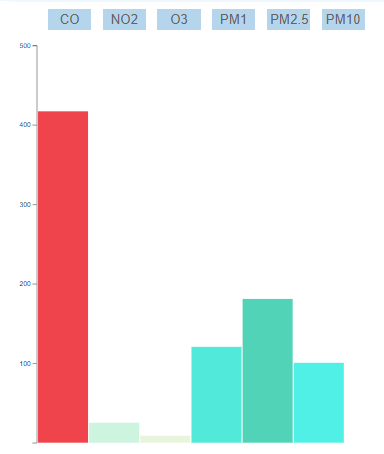
\includegraphics[width=5cm  ]{barchart}}
    \hfill
    \subfigure [Categoria medio ambiente]
       { 
\includegraphics[width=4cm]{unhealthyIcon}}
  
  \caption{Alert situation}
    \end{figure}

    Regarding the workflow, we are guiding the user from the selection of a point in the city of Malaga, either on his own initiative
    or automatic to the details of this point in real time and we continue to show  the evolution of the pollution at that point.
    The logic of this development is that it is anticipated that the user will be interested in the pollution that surrounds him in real time and if
    he wanta to know the breakdown of the pollutants at the point where he is, he can continue to inquire. The map, in addition to showing
    the point where the user is, serves as verification, gives more realism and confidence to the user.

\elsparagraph{Evaluation}  
\begin{itemize}
    \done The objective has been clearly defined and an investigation has been carried out, determining if the dataSet is appropriate.
    \done Worrying levels have been defined as poor, bad and unhealthy and are represented in the Air Guru tool. They stand out clearly so that the user is able to locate them quickly.
     \done The workflow is satisfactory, since the user knows the level of pollution at any location, at a simple glance. It is easy to explore the information further, if the user wishes.
         
\end{itemize}
 

\newpage
\subsection{Credibility and data quality}
It is essential that the credibility of the data set be impeccable. The source of the data must be reliable. In the description of the data, a section must be included where the origin of the data set is explained.

The quality of the data set can be measured according to the following characteristics of the values of the fields: \\
 
\textbf{Precision}. Units of measurement in the correct scale. For example, if we are measuring people's height, it would be meaningless to provide these measurements in meters, since the possible values will be 0, 1 and 2. \\

\textbf{Consistency}. Logical values for each type of field. An example would be a date field, all should
follow the same format. \\

\textbf{Interpretability}. Readable. The data must be clear, both in values and in units. For example, we can not
suppose the unit or scale of the data or, if the data set is dichotomous, "true" or "false", and the values represented are
"A" or "B", we can not assume true = A and false = B without this information being described. \\

\textbf{Complitud}. The data must be consistent in each of the samples. The samples can be differentiated
  from each other, as we see in the Figure below, can share some fields and not others. It would be
better to have a high degree of compliance for the data that interests us in our design.


\begin{figure}[ht]
\centering
\framebox{
\vbox{\begin{tabbing} 
Document \\
\hspace*{5mm} \= Sample 1 \\
\hspace*{10mm}\textit{Field A:} \hspace*{5mm} \= value A \\
\hspace*{10mm}\textit{Field B:} \hspace*{5mm} \= value B \\
\hspace*{5mm} \= Sample 2 \\
\hspace*{10mm}\textit{Field A:} \hspace*{5mm} \= value A \\
\hspace*{10mm}\textit{Field C:} \hspace*{5mm} \= value C \\
\hspace*{10mm}\textit{Field D:} \hspace*{5mm} \= value D \\
\hspace*{5mm} \= ... 
\hspace*{5mm} \= Sample n \\
\hspace*{10mm} \= ... 
\end{tabbing}}%
}
\caption{Example source source document}
\end{figure}

\subsubsection{How to solve it} 
The first step is to compare the information with the source of origin. With the data set and the definition
of each of the fields, the scale and interpretability of the fields and values must be checked.
Then we can perform different analysis of the data to check its consistency and compliance.
It is possible to use different graphs and see if there are extreme or strange values.
Database analysis tools can tell us the completeness of the fields, that is, what percentage of the
samples contain each field.

\subsubsection{How we solve it. Aire Guru} 
The source of data is verified by both the CEMI (Malaga information center) and UrbanClouds, the private company
that collects and sends the data to the city of Malaga.
With the description of the data in the open data portal of Malaga and the information received by UrbanClouds,
we obtain all the necessary information to interpret the data set. \\

For each field, a graphical study has been carried out with the Tableau tool and has verified that the values of the
fields meet the scale and range of expected values, that is, they are precise and consistent.
Using the analysis tools of MongoDBCompas and NoSQLBooster we verify the completeness of the fields needed for our model.
\begin{figure}[ht]
    \centering
    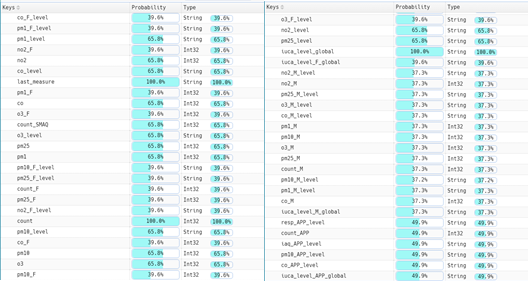
\includegraphics[width=12cm]{noSQLBoosterAnalysis}
    \caption{Completeness analysis}
\end{figure}

\elsparagraph{Evaluation}  
\begin{itemize}
    \done The necessary measures have been taken to verify and understand each of the fields in the data set.
    \done The values of each of the fields have been analyzed by checking scales and ranges.
    \done The completeness of the data has been analyzed.
    
\end{itemize}
 \newpage
\subsection{Enfoque al usuario}
Una gran parte del objetivo marcado en el apartado 3.1 Diseno, viene definido por el servicio que queramos ofrecerle
al usuario, ya que este, es nuestro cliente final y al que pretendermos ayudar.\\


Tendremos que definir las necesidades que muestran los usuarios en combinacion con las carencias del mercado.
Para ello tendremos que decidir si nuestro objetivo esta dirigido a un publico de gran dimension, por lo que tendremos que
que identificar las necesidades homogeneas del usuario medio o si el objetivo esta enfocado a un tipo de usuario
especifico, con necesidades caracteristicas.\\

Por lo tanto necesitamos un estudio actual sobre el nivel psicologico, social y economico del grupo objetivo, para descubrir, no solo
las necesidades, pero tambien los deseos, que le gustaria tener y sus demandas, que quieren.

Una vez los usuarios tengan acceso a los datos tal y como se los proporcionamos, es importante tener una retroalimentacion, 
seria ideal poder realizar un analisis del comportamiento del usuario para ve sus pautas respecto a los datos obtenidos.

\subsubsection{How to solve it} 
Es importante definir a que tipo de usuarios va dirigido. Estudiar tanto sus caracteristicas como la situacion del
mercado.
Utilizar un mecanismo que nos ayude a obtener una retroalimentacion, ya sea por un sistema de puntualizaciones, test o
un mecanismo automatico que permita conocer el comportamiento del usuario. Tambien podremos optar por la combinacion de ambas 
opciones.

\subsubsection{How we solve it. Aire Guru} 
Aire Guru va dirigido a toda la poblacion, por lo que tendremos en cuenta a la hora de implementarlo que la informacion debe
mostrarse de una forma simple, ademas de completa. Ademas, ponemos especial atencion a los usuarios que puedan tener una
enfermedad o condicion medica influenciada por la polucion del aire.
Durante el estudio de mercado, nos dimos cuenta, que muchas de ellas ofrecian la polucion del aire a tiempo real, pero 
pudimos ver las siguientes carencias:
\begin{itemize}
    \item Obsolete measurements. Measurements need to be taken regularly, since there can be huge differences
    between pollution levels at different times of the day.
    \item Limited geographic coverage. The data must cover a reasonable proportion of areas that people spend significant time in.
    \item Insufficiently granular measurements. Measurements must be at a reasonably fine level of granularity. One single measurement for an entire city is not useful.
    \item Poor presentation. Often the information is presented in an uninterpreted form, making it difficult for users to visualize, especially in a geographic sense.
    \item Poor discrimination and interpretation. Many tools show individual values as a number or a colour. This information is not
    enough for the user to take control of their exposure. Such visualizations are not really compelling. 
    \item Exposicion a la polucion de una forma personalizada. Nos interesa saber a que nivel de polucion estamos expuesto
    a lo largo del tiempo, no de forma puntual.
    \item Necesidad de utilizar complicated devices para monitorizar la exposicion. Nuestro objetivo es facilitar la informacion a los 
    usuarios con el minimo de complicaciones posibles.
    \item Sin informacion dedicada por condicion medica. 
\end{itemize}

Una vez implementado, probamos la aplicacion con 14 usuarios. Nuestra herramienta integra Google Analytis que nos permite saber el 
comportamiento de los usuarios, como a cuantas paginas acceden, a cuales y cuanto tiempo permanencen en ella. Ademas, finalizada la prueba,
se realizo una encuesta para medir no solo el nivel de satisfaccion, pero tambien para comprobar la utilidad y si habia conseguido el objetivo.
\begin{figure}[ht]
    \centering
   \subfigure[Aire Guru Form]
    {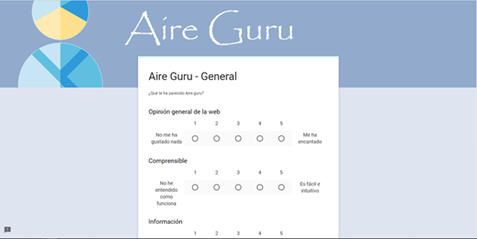
\includegraphics[width=5.5cm  ]{form}}
    \hfill
    \subfigure [Google Analytics]
       { 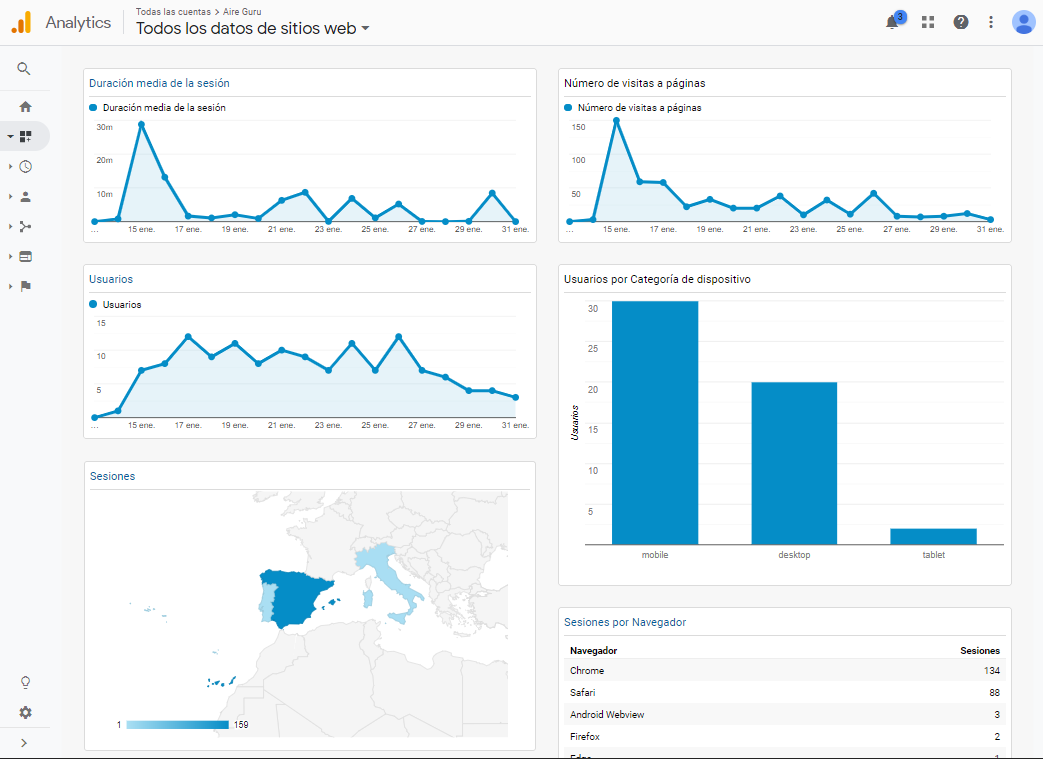
\includegraphics[width=5.5cm]{googleAnalytics}}
  
  \caption{User Feedback}
    \end{figure}
 
\elsparagraph{Evaluation}  
\begin{itemize}
    \done El estudio de mercado nos hizo ver con claridad las carencias que existen en las aplicaciones actuales.
    \done La encuesta nos reporto valoraciones muy positivas respecto a la utilizacion, comprension e informacion reportada.
    \done Usuarios nos comentaron que gracias a Aire Guru habian descubierto que tenian una condicion medica que se puede ver afectada por
    la polucion del aire

\end{itemize}
 

\newpage
\subsection{Util}
Usualmente cometemos el error de intentar mantener al usuario lo mas informado posible y le ofrecemos datos que
no aportan informacion nueva, es redundate.
Debemos centrarnos en que nuestro objetivo no es crear usuarios especializados en la materia, sino aportarles la
informacion de una manera que la puedan aplicar a su vida diaria y asi mejorarla, por lo que huiremos de datos
tecnicos, dificiles de interpretar.

Como mencionamos anteriormente, huiremos de toda aquella informacion vana, que no haga ninguna aportacion
al objetivo marcado. No queremos que el usuario se distraga o se pierda en medio de una piscina de datos completa
pero compleja que para el no tenga ningun sentido. 

Respecto a la representacion, debe seguir el mismo principio, huiremos de decoraciones inecesarias que hagan al 
usuario perderse, solo debe contener la informacion necesaria para poder ser interpretada correctamente, es decir,
toda representacion tienen que contarnos lo que significa sin tener que estar accediendo continuamente a informacion
extra.

En caso complejos, los conceptos que no sean de uso diario para los usuario, podremos poner informacion
complementaria a su disposicion para que el usuario pueda informarse sobre el significado de los datos 
representados, esta practica proporcionara al usuario un mayor dominio del concepto y podra estar mas
seguro de su lectura de los datos, ya que cuando dirigimos al usuario a fuentes oficiales de informacion, donde puedan 
obtener una explicacion veridica,reenforzamos la credibilidad de las representaciones que estamos realizando. En todo caso, 
fuera de la representacion principal, porque el usuario no tendra que acceder a esta informacion continuamente.

\subsubsection{How to solve it} 
Centrarnos en el objetivo, mostrar los datos directamente relacionados con nuestra meta, no annadir los datos 
simplemente porque aparezcan en el conjunto de datos, y no annadir detalles tecnicos irrelevantes para el usuario.


\subsubsection{How we solve it. Aire Guru} 
No util - identificacior de la estacion de medida
 Nos centramos en 6 contaminantes y la medida es unica para todos y el general, el AQI, los rangos son exactamente
 los mismos para todos
 No existen datos que el usuario no entienda, como coordenadas, identificador de la estacion, como se ha tomado la medida.
 Si la medida no existe, simplemente la obviaremos.

\elsparagraph{Evaluation}  
\begin{itemize}
    \done Se ha eliminado la informacion no relevante para el usuario.
    \crossed Se han ofrecido las mediciones exactas. Estos datos son demasiado tecnicos para el usuario. Sin embargo,
    aporta veracidad a los datos y se han  posicionado en un lugar secundario para que no distraiga al usuario.
    
\end{itemize}
 \newpage
\subsection{Personalizacion}
 
    --relevante de manera general vs relevante personal
    --casos personales
    --aplicabilidad
    --solventar problema en particular
    
    
    
    \begin{itemize}
    
          \item Herramientas necesarias para que el usuario entienda la informacion y de porque
     \item conocimientos multidisciplinares
        \item fuentes fiables, actualizacion periodica
    \end{itemize}
  

\subsubsection{How to solve it} 


\subsubsection{How we solve it. Aire Guru} 
 
\elsparagraph{Evaluation}  
\begin{itemize}
    \done
    \crossed
    
\end{itemize}
 \newpage
\subsection{Check List}

\begin{figure}[ht]
  \centering
  \framebox{
  \vbox{\begin{tabbing} 
 
  \hspace*{10mm} \ding{47} Point 1 \hspace*{25mm} \= \ding{47} Point B \hspace*{25mm} \= \ding{47} Point B\\
   
  \end{tabbing}}%
  
  }
  \end{figure} 
\newpage
\section{Compelling}
\subsection*{}
Una vez demostrada la relevancia, beneficios y ventajas de la utilizacion de los datos por parte del usuario, es necesario un trabajo minucioso para
transmitir estos conceptos al usuario de forma clara, sencilla y directa y asi lograr un vinculo que haga crecer el deseo del usuario de profundizar en la materia y
mantenerse informado. 
Solo si el usuario entiende la relevancia de los datos y la influencia que estos tienen en su vida diaria, sera posible un compromiso por parte de este.

Para conseguir este objetivo, es importante reflejar la informacion de una manera atractiva tanto desde un punto de vista conceptual como funcional, 
es decir, dejando claro la implicacion de los datos y reflejandolos con una correcta presentacion, que guie al usuario de una manera logica y estructurada.

Desde un punto de vista conceptual, la informacion debera cubrir una necesidad del usuario, aunque el usuario no sepa a priori que tiene esta necesidad.
Es decir, aqui entra en juego la representacion de la informacion de una manera que despierte la necesidad de monitorizacion de los datos por parte
del usuario.

[....].
\begin{itemize}

\item usuario no sabe que tiene la necesidad
\item necesidad para el usuario
\item fundamental para la vida diaria
\item mejora para sus tareas diarias
\item personalizacion
\item Ligar la informacion a la resolucion de problemas comunes
\item \end{itemize}

Desde un punto de vista funcional se ha de tener en cuante, que para lograr el mayor alcance de usuarios, de distintos tipos, se han
de repetar las siguientes premisas,  la informacion debe ser presentada en un formato facil de entender por
el usuario, de una forma logica, que respete un order, es decir, de menos detalles a mas, que le de la posibilidad al usuario de indagar por si mismo, como
si la redaccion de una novela se tratara.
La representacion debe estar fuera de toda ambiguidad, no mostrar informacion que resulte enganosa o que haya que dedicar demasiado tiempo fijandonos
en los detalles para poder interpretarla correctamente.
Ademas se debera buscar la manera de presentar la informacion de una manera armonica y agradable para el usuario.
Al represnentar la informacion sera incluido lo basicamente necesario, huyendo siempre de graficas recargadas que solo aporten ruido a la represetacion.


\begin{itemize}
\item facil de entender
\item Analisis del publico al que va dirijido
\item agradable
\item no enganar
\item nivel alto de detalle sin datos personales
\item actual
\item Herramientas necesarias para que el usuario entienda la informacion y de porque
\item formato adecuado para un amplio espectro de usuarios
\item Crear familiaridad
\item Flexibilidad de seleccion de subdata
\item No decoracion que ensucie o distraiga de la informacion principal
\item Consecuente, que siga una secuencia logica
\item Estudio de las representaciones mas adecuadas para cada tipo de datos
  \end{itemize}
\subsection*{}
\subsection*{} 
\newpage
\section{Evaluation}
\begin{itemize}
   \item  { Methodology, Results } / 
   \item   -Enquete, real test results...
   \item   -Analysis of the results   
   \item   Podemos entender  que significa cada uno de los campos representados en el conjunto de dato gracias a la informacion
   complementaria presentada en el portal de datos abiertos y por la informacion proporcionada por la empresa encargada de 
   recolectar los datos.
\end{itemize}
 
\section*{Conclusion}
\begin{itemize}
    \item -General conclusion,
    \item recapitulation,
    \item main points,
    \item future work,
    \item where is available
\end{itemize} 
\newpage
\section{References}

Braidot, N.P. (2009). Neuromarketing. Ediciones Gestión 2000.\\

Burton, B., Geishecker, L., Hostmann B, Friedman, T. y Newman, D. (2006).
Organizational Structure: Business Intelligence and Information Management.
Gartner.\\

Cano, J. L. (2007). Business intelligence: competir con información. Madrid:
ESADE Business School.\\


Chiasson, T.; Gregory, D. et al. (2014). A simple introduction to preparing and
visualizing information. Columbia, Missouri: Donald W. Reynolds Journalism
Institute and Infoactive.\\

Chiasson, T.; Gregory, D. et al. (2014). DATA + DESIGN A simple introduction to
preparing and visualizing information. Columbia, Missouri: Donald W. Reynolds
Journalism Institute and Infoactive. \\

Chakrabarti, S. (2003). Mining the Web: Discovering Knowledge from Hypertext Data.
California. Morgan Kaufmann.\\

Davenport, T., and Prusak, L. (2000). Working Knowledge: How Organizations Manage
What They Know. Massachuset: Harvard Business Review Press.\\

Davenport, T. H., Barth, P. y Bean, R. (2012). How big data is different. MIT Sloan
Management Review.\\

Debenham, J. (1998) Knowledge Engineering. Unifying Knowledge Base and Database
Design. Sydney: Springer.\\

Devlin, B. (1997). Data Warehouse: From Architecture to Implementation. Estados
Unidos: Addison-Wesley.\\

Eckerson, W. y White. C., (2003). Evaluating ETL and Data Integration Platforms.
TDWI Report Series.\\

Few, S. (2012). Show me the Numbers. Burlingame, California: Analytics Press.
Meirelles, I. (2013). Design for Information. Beverly, Massachusetts: Rockport
Publishers.\\

Han, J., Kamber, M. y Pei, J. (2006). Data Mining, Concepts and Techniques (2º
edición). Massachusets: Morgan Kaufmann.\\

Jarke, M., Jesusfeld, M.A., Quix, C., and Vassiliadis, P. (1998). Arquitecture and Quality
of Data Warehouses: An Extended Repository Approach. Advanced Information Systems
Engineering, Lecture Notes in Computer Science.\\

Kerin, R. (2014). Marketing. McGraw Hill. 

Kirk, A. (2012). Data Visualization: A sucessfull Design Process. Birmingham (UK):
Packt Publishing.

Lin, T. Y. (2002). Attribute transformation for data mining I: theoretical explorations.
International Journal of Intelligent Systems.\\

Markham, K. (2018). A Practical Guide to the General Data Protection Regulation (GDPR).Law Brief Publishing \\

Muñiz, R. (2014). Marketing en el siglo XXI. Centro de estudios financieros. \\

Murray, S. (2013). Interactive Data visualization for the Web. Massachusetts (EUA):
O’Reilly.\\

Parasurman, A. Zaithaml, V. A. y Berry, L. L. (1998). Servqual: a multiple-item scale for
mesauring consumer perceptions of service quality. Journal of Retailing.\\ 

Pettersson, R. (2013). Information Design 4- Graphic Design. Austria: International
Institute for Information Design (IID).\\

Redman, T.C. (1996). Data Quality for the Information Age, p. 245-267. Massachusetts:
Artech House, Inc.\\

Solomon, M.R. (2013). Comportamiento del consumidor. Addison-Wesley.\\

Telea, A. C. (2014). Data Visualization: Principles and practice, second Edition. Ohio
(EUA): CRC Press. \\

Tufte, E. R. (2001). The Visual Display of Quantitative Information. Cheshire,
Connecticut: Graphic Press.\\

Ware, C. (2013). Information Visualization. Waltham, Massachusetts: Morgan
Kaufmann Publishers. \\

Weller, K. (2010). Knowledge Representation in the Social Semantic Web. New York:
De Gruyter. \\


 

\end{document}
  
